\documentclass[11pt,a4paper]{article}
\usepackage[margin=0.9in]{geometry}


\usepackage{graphicx,booktabs,array,tabularx,xcolor,enumitem,amsmath,float}
\usepackage[colorlinks=true,linkcolor=blue!50!black,urlcolor=blue!50!black]{hyperref}
\usepackage{titlesec,fancyhdr}
\definecolor{accent}{HTML}{1F4E79}
\titleformat{\section}{\large\bfseries\color{accent}}{\thesection}{0.6em}{}
\titleformat{\subsection}{\normalsize\bfseries\color{accent}}{\thesubsection}{0.5em}{}
\titlespacing*{\section}{0pt}{11pt}{4pt}
\titlespacing*{\subsection}{0pt}{7pt}{2pt}
\setlist{nosep,leftmargin=1.3em}
\setlength{\parskip}{3pt}\setlength{\parindent}{0pt}
\pagestyle{fancy}\fancyhf{}
\fancyhead[L]{\small RiskPulse --- S\&P Global \& Crisil Campus Hackathon 2026}
\fancyhead[R]{\small Shusmit Sarkar}
\fancyfoot[C]{\small\thepage}
\renewcommand{\headrulewidth}{0.3pt}
\sloppy\emergencystretch=2em
\newcolumntype{P}[1]{>{\raggedright\arraybackslash}p{#1}}
\newcolumntype{Y}{>{\raggedright\arraybackslash}X}
\begin{document}

\begin{center}
{\LARGE\bfseries\color{accent} RiskPulse}\\[3pt]
{\large AI/NLP Risk Engine with Event-Driven Portfolio Stress Testing (Module B)}\\[6pt]
{\small \textbf{Candidate:} Shusmit Sarkar \quad \textbf{Institute:} IIT Kharagpur \quad \textbf{Email:} shusmit.sarkar@gmail.com\\
\textbf{Repository:} \url{https://github.com/SHUSMIT/spglobal}}
\end{center}
\vspace{-4pt}\hrule\vspace{4pt}


\section{Problem Context and Walkthrough}
\textbf{The situation.} Wholesale banking risk teams monitor thousands of headlines, wire stories and event records every day. Market-moving information---a sanctions announcement, a counterparty downgrade, a central-bank surprise, a cyber incident---appears first as unstructured text. Today that text is read manually or filtered by keyword alerts, which creates three gaps: alerts are not ranked by severity, they are not classified in a consistent taxonomy, and they are not connected to the bank's own exposures. The result is slow triage and an unclear answer to the question that matters: \emph{what does this event do to our book?}

\textbf{How I read the problem statement.} The case study has two layers. The first is a reusable AI/NLP Risk Engine that ingests text from at least two sources and emits, per article, a sentiment score, an event class and an impact score in machine-readable form. The second is a downstream module that consumes those signals. Module A (a tactical index rebalancer) acts on sentiment alone; Module B (a strategic stress tester) acts on event class and impact score and needs a portfolio model. I chose \textbf{Module B} because it exercises all three engine outputs, ties them to quantified portfolio consequences, and matches how wholesale-banking risk functions actually use event intelligence.

\textbf{Approach in five steps.}
\begin{enumerate}[leftmargin=1.5em]
\item \emph{Ingest} headlines and summaries from Google News RSS and GDELT DOC~2.0 (NewsAPI and CSV upload are also supported) into one schema.
\item \emph{Understand} each article: FinBERT sentiment, an event class from domain terms plus MiniLM semantic similarity, matched entities, and a learned impact score.
\item \emph{Gate} on severity: only events with impact $\ge 7$ trigger a stress scenario.
\item \emph{Transmit} the event through a mixed portfolio using explicit shocks for equity, rates, spreads and default probability.
\item \emph{Present} signals, scenarios and position-level losses through an API and a dashboard, with CSV export.
\end{enumerate}

\begin{table}[H]
\centering\small
\begin{tabularx}{\linewidth}{@{}P{3.2cm}P{4.3cm}Y@{}}
\toprule
\textbf{Design decision} & \textbf{Choice} & \textbf{Rationale}\\
\midrule
Language models & Frozen FinBERT and MiniLM & Strong financial-text representations without training cost; stable, reproducible inference\\
Event taxonomy & 10 classes + Other, terms plus class descriptions & Domain terms keep labels interpretable; embeddings handle paraphrase\\
Impact definition & Predicted next-day absolute price move, scaled 1--10 & Ties severity to observed market reaction rather than hand-set weights\\
Stress method & Explicit shock vectors per event class & Transparent and auditable; every loss traces to a sensitivity\\
Trigger & Impact score $\ge 7$ & Matches the case-study example; limits stress runs to material events\\
Interfaces & FastAPI, React dashboard, CSV & Engine output consumable by any downstream application\\
\bottomrule
\end{tabularx}
\caption{Key design decisions and their rationale.}
\end{table}

\section{System Design}
\begin{figure}[H]
\centering
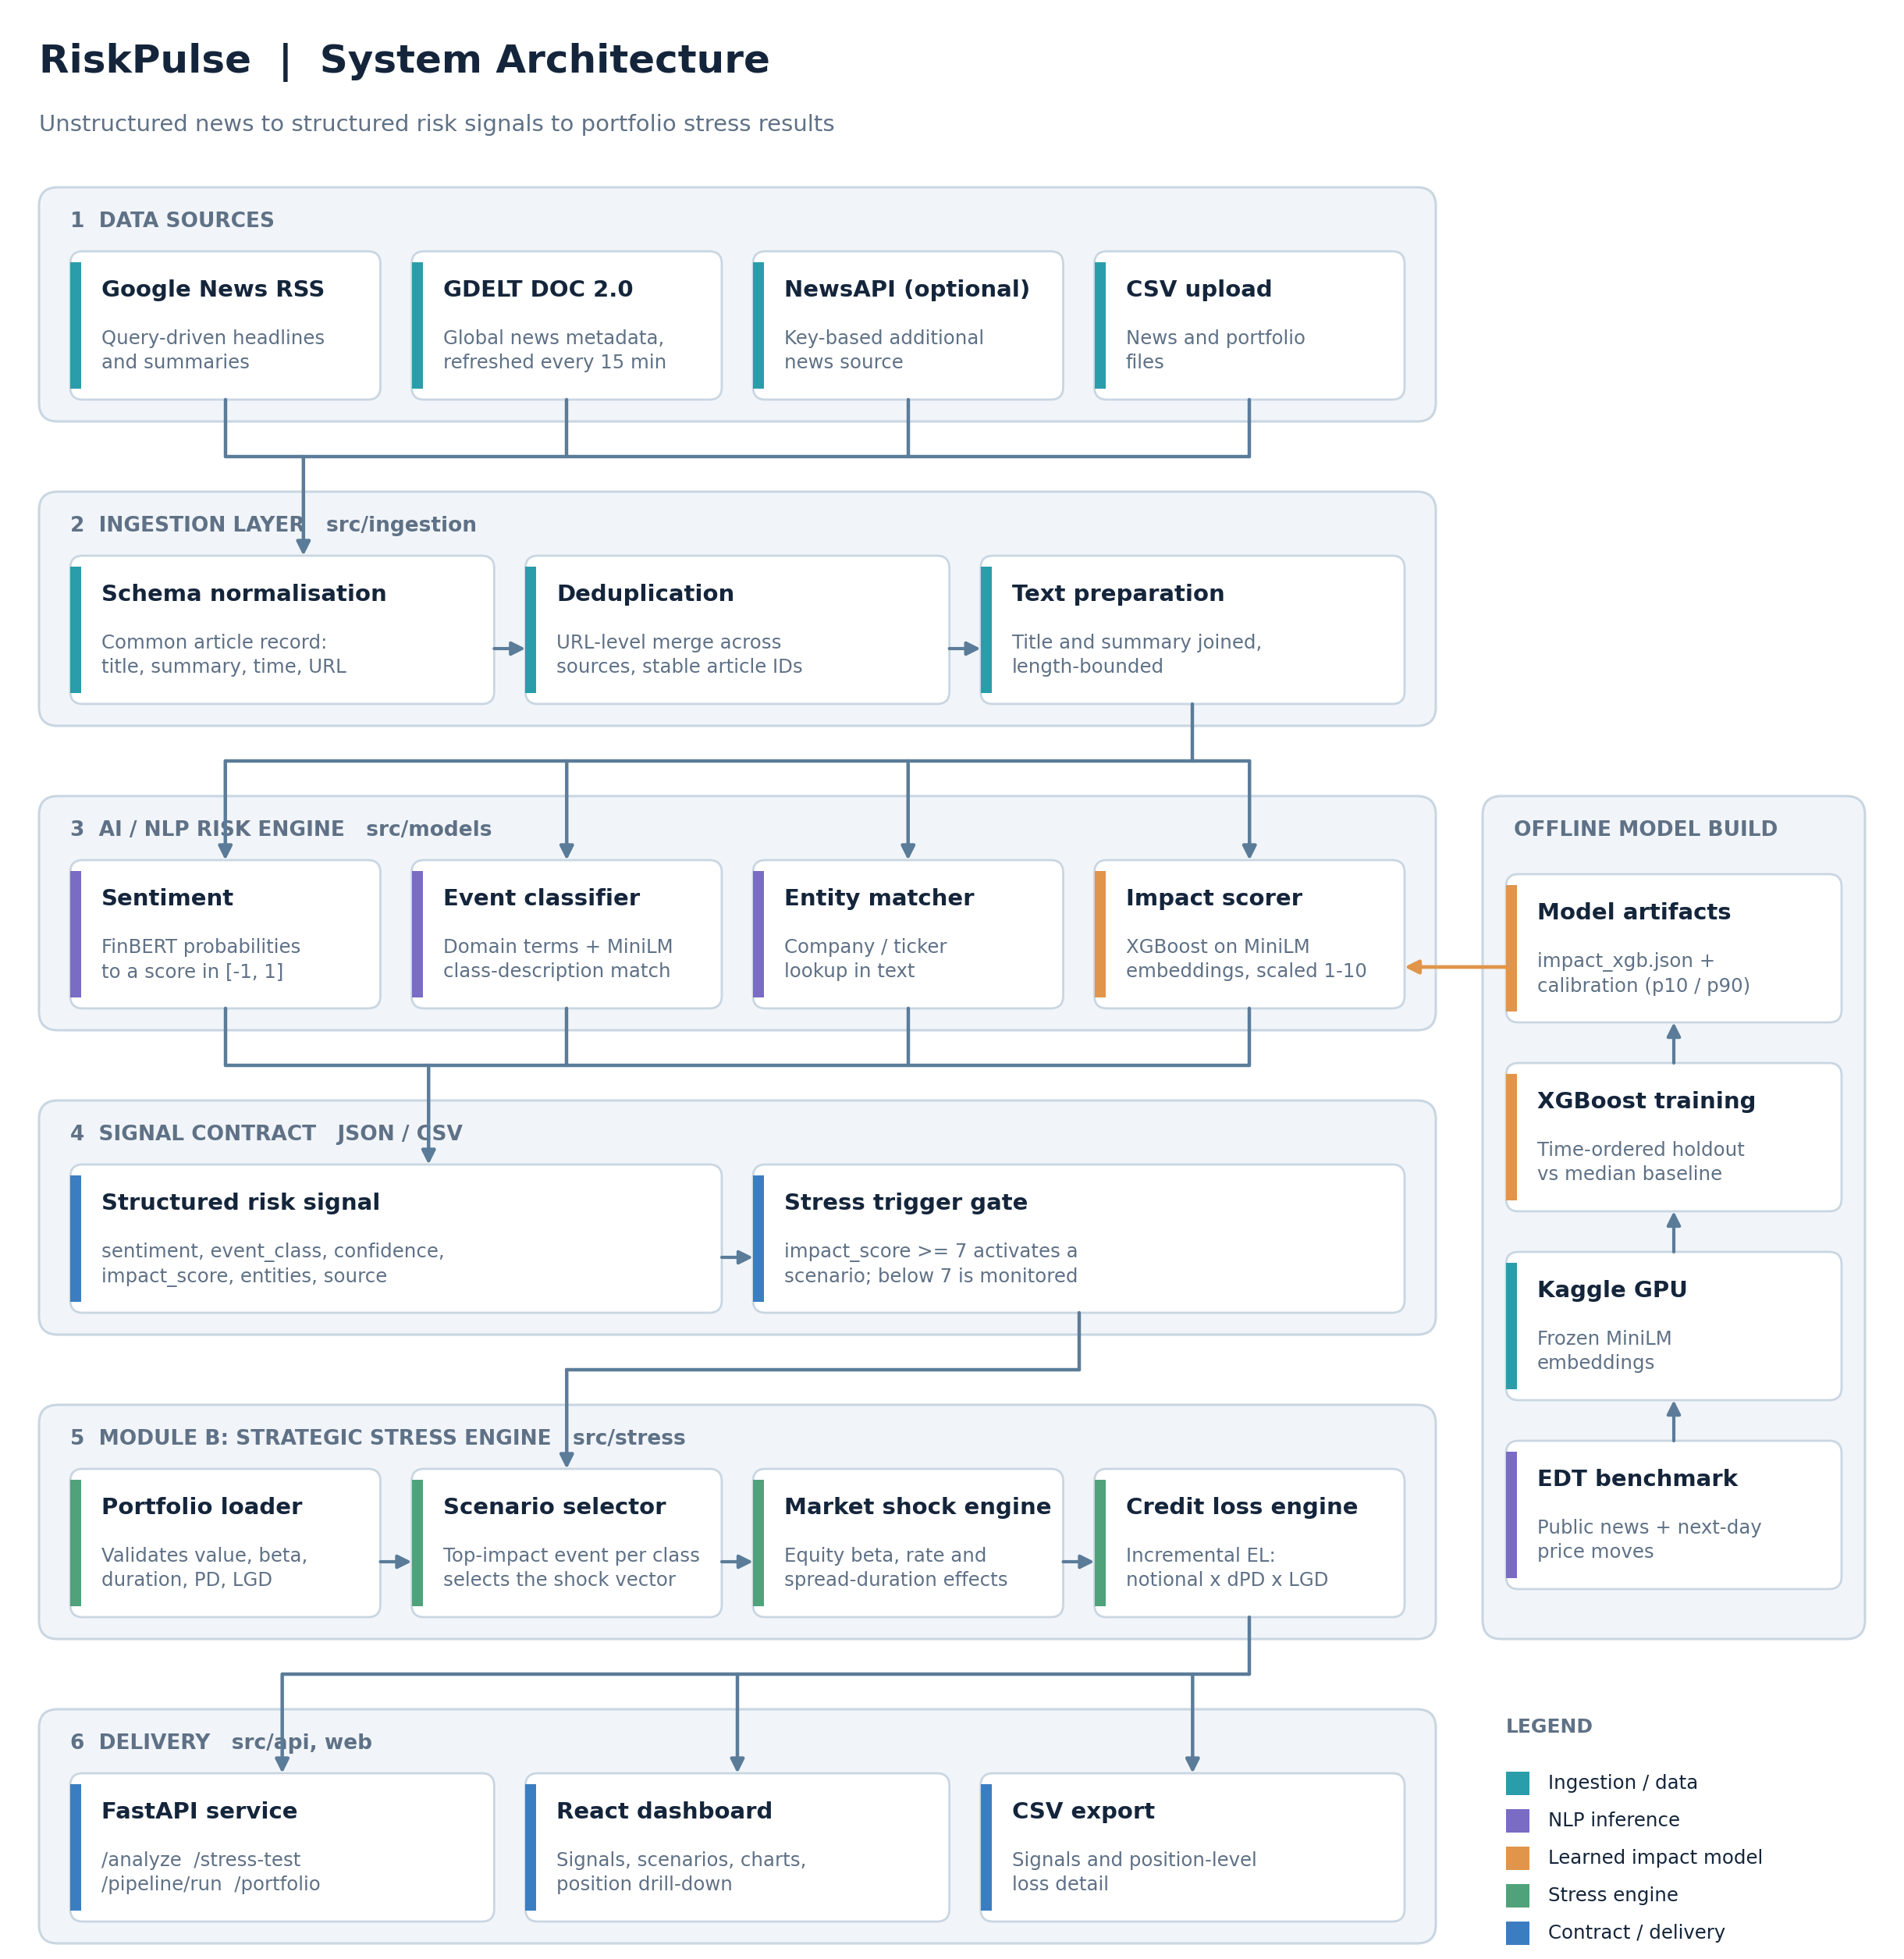
\includegraphics[width=0.84\linewidth]{architecture.png}
\caption{RiskPulse layered architecture: sources, ingestion, NLP risk engine, signal contract, Module B stress engine and delivery. The offline lane trains the impact model whose artifacts are loaded by the impact scorer.}
\end{figure}

Data moves top to bottom through six layers. Sources are normalised into a common article record and deduplicated by URL. The text is passed in parallel to the sentiment, event-classification, entity-matching and impact components, whose outputs are merged into one structured signal. A trigger gate passes events with impact $\ge 7$ to Module B, which loads and validates the portfolio, selects the scenario for each event class, applies market shocks and credit-loss increments, and returns before/after values to the API, dashboard and CSV export. Code is organised by layer: \texttt{src/ingestion}, \texttt{src/models}, \texttt{src/stress}, \texttt{src/services}, \texttt{src/api} and \texttt{web/}.

\section{Data Sources and Provenance}
All data is public or generated by the author; no proprietary or client data is used.
\begin{table}[H]
\centering\small
\begin{tabularx}{\linewidth}{@{}P{3.3cm}P{3.6cm}Y@{}}
\toprule
\textbf{Dataset / feed} & \textbf{Nature} & \textbf{Use in the system}\\
\midrule
Google News RSS & Public, query-driven headlines and summaries & Live news source for the engine\\
GDELT DOC 2.0 & Public global news metadata & Second live source; broadens event coverage\\
EDT benchmark & Public news with next-day price labels & Training and validation of the impact model\\
\texttt{portfolio.csv} & Generated, 12 positions, 5 asset types & Module B portfolio with beta, duration, PD, LGD\\
\texttt{sample\_\allowbreak news.csv} & Generated news records across event types & End-to-end pipeline runs and tests\\
\texttt{public\_\allowbreak news\_\allowbreak snapshot.csv} & 30 public RSS headlines & Reproducible inspection of live-source output\\
\texttt{entity\_\allowbreak universe.csv} & Public company--ticker lookup & Entity matching and related-news linkage\\
\bottomrule
\end{tabularx}
\caption{Datasets, provenance and purpose (files are in \texttt{data/}; training artifacts in \texttt{models/}).}
\end{table}

\section{AI/NLP Risk Engine}
\textbf{Ingestion.} Each run issues one bounded request per configured source and merges the results by URL. Uploaded news CSVs follow the same schema (\texttt{article\_id, published\_at, source, publisher, title, summary, url, query}), so live and file-based inputs are processed identically.

\textbf{Sentiment.} FinBERT (\texttt{ProsusAI/finbert}) class probabilities are converted to a signed score in $[-1,1]$ and a positive/neutral/negative label. A financial lexicon scorer supplies the same output fields where the transformer is not loaded, so the schema is stable in every environment.

\textbf{Event classification.} Ten classes are supported: Geopolitical, Macroeconomic, Credit Event, Merger/Acquisition, Product Launch, Regulatory/Legal, Earnings/Guidance, Market Liquidity, Operational/Cyber and Commodity/Supply Chain, with \emph{Other} for unmatched text. Curated domain terms (for example \emph{sanctions}, \emph{default}, \emph{ransomware}) are combined with cosine similarity between the MiniLM embedding of the article and a short reference description of each class. Explicit domain evidence is kept unless the semantic match disagrees with high confidence. Every label carries a confidence value.

\textbf{Impact score.} The impact model predicts the absolute next-trading-day price move of the referenced stock from the article's MiniLM embedding. Training used the public EDT news--market benchmark: 50{,}000 of 75{,}395 valid records, split chronologically into 40{,}000 training rows and 10{,}000 later validation rows. Embeddings were computed on a Kaggle GPU and an XGBoost regressor was trained on the log-transformed move. Predictions are scaled linearly to 1--10 between the training 10th and 90th percentile moves (0.095\% and 6.52\%). The model and calibration are stored in \texttt{models/}.

\begin{table}[H]
\centering\small
\begin{tabular}{@{}lccc@{}}
\toprule
\textbf{Time-ordered validation (10{,}000 rows)} & \textbf{MAE (pp)} & \textbf{RMSE (pp)}\\
\midrule
XGBoost on MiniLM embeddings & \textbf{1.699} & 3.224\\
Train-median baseline & 1.731 & ---\\
\bottomrule
\end{tabular}
\caption{Impact-model validation on later-dated data; the model improves on the baseline out of time.}
\end{table}

\section{Module B: Strategic Portfolio Stress Testing}
\textbf{Portfolio.} The portfolio contains 12 positions worth USD 105.12\,million: 3 loans (35.20m), 3 bonds (24.95m), 2 derivatives (16.82m), 3 equities (23.25m) and 1 consumer credit pool (4.90m). Each position records value, notional, opening/closing value, P\&L, equity beta, rate duration, spread duration, PD and LGD. A portfolio CSV with these columns can be uploaded and is validated on load.

\textbf{Shocks.} Each event class maps to a shock vector applied at full severity:

\begin{table}[H]
\centering\small
{\footnotesize\setlength{\tabcolsep}{3.2pt}\begin{tabular}{@{}lrrrr@{\hspace{0.5cm}}lrrrr@{}}
\toprule
\textbf{Event class} & \textbf{Eq.} & \textbf{Rate} & \textbf{Sprd} & \textbf{PD$\times$} & \textbf{Event class} & \textbf{Eq.} & \textbf{Rate} & \textbf{Sprd} & \textbf{PD$\times$}\\
\midrule
Geopolitical & $-10\%$ & +75bp & +150bp & 1.35 & Operational/Cyber & $-5\%$ & +25bp & +100bp & 1.35\\
Macroeconomic & $-8\%$ & +200bp & +100bp & 1.30 & Commodity/Supply & $-6\%$ & +100bp & +125bp & 1.25\\
Credit Event & $-6\%$ & +100bp & +250bp & 2.00 & Earnings/Guidance & $-5\%$ & +25bp & +75bp & 1.15\\
Market Liquidity & $-8\%$ & +75bp & +200bp & 1.50 & Merger/Acquisition & $+3\%$ & $-25$bp & $-50$bp & 0.95\\
Regulatory/Legal & $-7\%$ & +50bp & +125bp & 1.25 & Product Launch & $+3\%$ & 0bp & $-25$bp & 0.98\\
\bottomrule
\end{tabular}}
\caption{Event-specific shocks (equity return, rate move, spread move, PD multiplier).}
\end{table}

\textbf{Loss calculation.} For impact score $s\ge7$ shocks are scaled by $k=s/10$ (PD multiplier $1+(m-1)k$). For position $i$ with value $V_i$, beta $\beta_i$, duration $D_i$, spread duration $S_i$ and notional $N_i$:
\begin{align*}
f_i &= 1 + \beta_i\Delta_{\text{eq}} - D_i\Delta_{\text{rate}} - S_i\Delta_{\text{spread}}, \qquad
\Delta\text{EL}_i = N_i\bigl(\min(PD_i m,0.95)-PD_i\bigr)LGD_i,\\
V_i^{\text{stressed}} &= V_i f_i - \Delta\text{EL}_i \quad(\Delta\text{EL}\text{ applies to loans, bonds and credit exposures}).
\end{align*}
Scores below 7 leave values unchanged. The engine returns baseline and stressed value, absolute and percentage loss, the applied shocks and a position-level table.

\section{Dashboard and API}
The React/Vite dashboard offers source selection (sample set, live Google News and GDELT, uploaded CSV), lookback and article-count controls; a severity-ranked signal table with sentiment, event type and stress status; an event-composition chart; a scenario selector showing the driver article and shocks; baseline versus stressed portfolio value; a position-level loss chart with drill-down to sensitivities, P\&L, credit loss and related news; and CSV export. An optional LLM analyst answers free-form questions over the analysed news. The same functions are available through \texttt{/analyze}, \texttt{/stress-test}, \texttt{/pipeline/run}, \texttt{/portfolio} and \texttt{/health}.

\section{Results}
Every article produces \texttt{sentiment}, \texttt{sentiment\_label}, \texttt{event\_class}, \texttt{event\_confidence}, \texttt{impact\_score} and \texttt{triggered\_stress}. Table~\ref{tab:res} shows portfolio outcomes at severity 8.

\begin{table}[H]
\centering\small
\begin{tabular}{@{}lrrrr@{}}
\toprule
\textbf{Event class (severity 8)} & \textbf{Before (USD m)} & \textbf{After (USD m)} & \textbf{Loss (USD m)} & \textbf{Loss (\%)}\\
\midrule
Macroeconomic & 105.12 & 93.54 & 11.58 & 11.02\\
Credit Event & 105.12 & 93.78 & 11.34 & 10.79\\
Geopolitical & 105.12 & 94.49 & 10.63 & 10.11\\
Market Liquidity & 105.12 & 94.63 & 10.49 & 9.98\\
Regulatory/Legal & 105.12 & 97.39 & 7.73 & 7.35\\
Operational/Cyber & 105.12 & 99.49 & 5.63 & 5.36\\
Merger/Acquisition & 105.12 & 108.34 & $-3.22$ & $-3.07$\\
\bottomrule
\end{tabular}
\caption{Module B outcomes per event class. A negative loss is a gain.}\label{tab:res}
\end{table}

\begin{figure}[H]
\centering
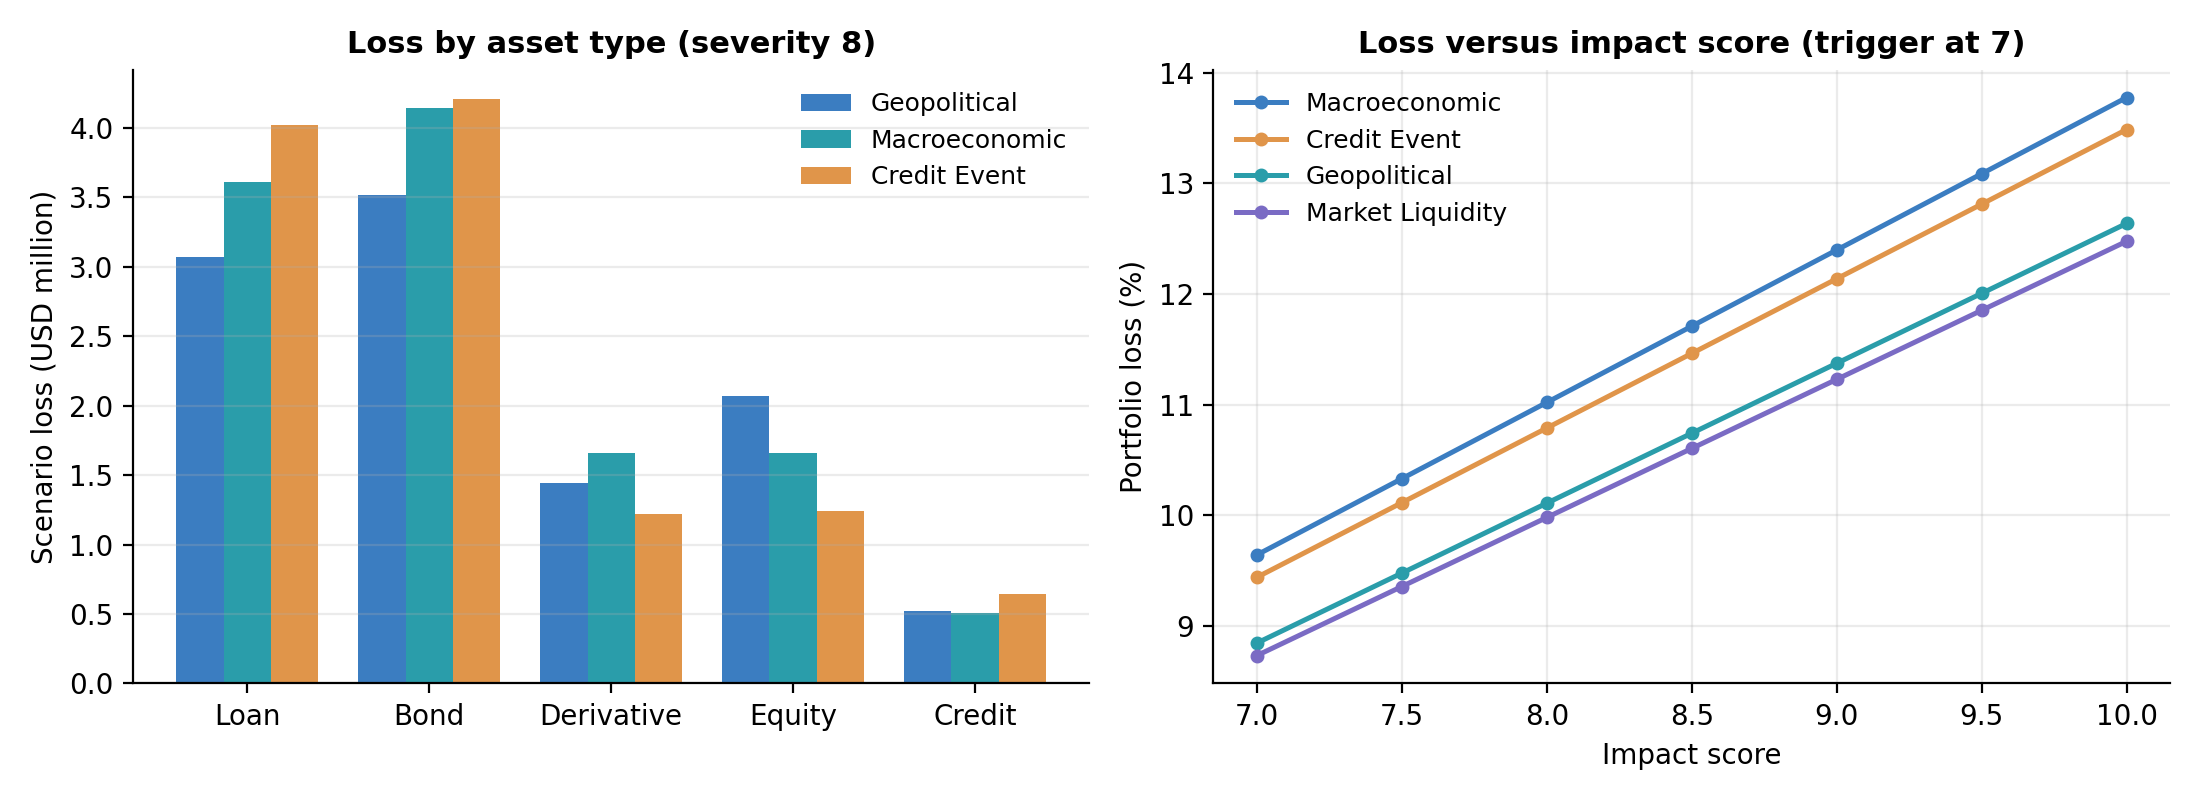
\includegraphics[width=\linewidth]{results.png}
\caption{Left: loss by asset type under three high-impact events. Right: portfolio loss as the impact score rises from the trigger of 7 to 10.}
\end{figure}

The results separate event types in an interpretable way. Credit events concentrate losses in loans and bonds through the doubled PD multiplier and wide spread shock (loan L003 loses USD 2.09m and bonds B001--B003 lose 1.53m, 1.45m and 1.22m); geopolitical events weigh most on equities; macroeconomic events act mainly through rate duration. Loss grows monotonically with severity above the trigger, and positive corporate events produce a net gain. Against a keyword-alert workflow, which flags headlines but gives no severity order or portfolio consequence, the pipeline returns a ranked signal list, a selected driver event per class, the stressed value and the most affected positions in one run. The automated test suite covers the health endpoint, sample and uploaded-news pipelines, the trigger at 7, the below-trigger case, API input bounds and coverage of every asset type.

\section{Domain Impact}
\begin{itemize}
\item \textbf{Faster, consistent triage:} analysts review a classified, severity-ranked list rather than raw feeds.
\item \textbf{Exposure-aware alerts:} each trigger shows which loans, bonds, derivatives and equities are affected and by how much.
\item \textbf{Governance:} shocks, threshold and sensitivities are explicit and can be challenged or recalibrated by a risk officer.
\item \textbf{Reusability:} the JSON/CSV signal contract supports other consumers, such as a sentiment-driven rebalancer, and an institution's own portfolio without engine changes.
\end{itemize}

\section{Assumptions, Limitations and Next Steps}
\begin{table}[H]
\centering\small
\begin{tabularx}{\linewidth}{@{}P{3.1cm}YY@{}}
\toprule
\textbf{Area} & \textbf{Assumption / basis} & \textbf{Implication and next step}\\
\midrule
Portfolio data & No organiser transaction file was supplied, so a 12-position wholesale-style portfolio was generated; it contains no client data & Any institutional portfolio CSV with the required columns can be loaded unchanged\\
Scenario shocks & Analyst-defined shock vectors per event class, scaled by severity & Results are scenario analysis, not forecasts; calibrate against historical crisis episodes\\
Impact score & Market-movement proxy for single-stock next-day moves from the EDT benchmark & Not a causal loss estimate; extend with more periods and full-text features\\
Entity mapping & Name-to-ticker lookup over a compact public universe & Imperfect matches possible; add validated issuer and counterparty mappings\\
News content & Headlines and summaries from public feeds; coverage varies by source and query & Add full-text retrieval and further sources\\
Trigger threshold & Impact $\ge 7$, as in the case-study example & Make the threshold and scaling configurable per desk\\
Scope & Module B implemented; Module A not built & Reuse the sentiment signal for a tactical rebalancer\\
\bottomrule
\end{tabularx}
\caption{Assumptions, their implications and planned extensions.}
\end{table}

\section{Conclusion}
RiskPulse delivers the complete chain the case study asks for: a multi-source AI/NLP Risk Engine producing sentiment, event class and impact score, and a Module B stress tester that turns those signals into quantified, position-level portfolio consequences. Design choices favour transparency---frozen language models, a learned and validated impact score, explicit shocks and a documented trigger---so that every output can be inspected, challenged and recalibrated. The same signal contract leaves room to add further downstream applications without changing the engine.

\end{document}
